%%%%%%%%%%%%%%%%%%%%%%%%%%%%%%%%%%%%%%%%%%%%%%%%%%%%%%%%%%%%%%%%%%%%%%%%%%%%%%%
%%  Multimedia Computing — Progress Report
%%  Project : Speech-to-Text Generation with OpenAI Whisper
%%  Author  : [Your Name]   (Student ID: [Your ID])
%%  Course  : [Course Code] — Multimedia Computing
%%  Instr.  : Ali Altan
%%  Term    : Spring 2026
%%%%%%%%%%%%%%%%%%%%%%%%%%%%%%%%%%%%%%%%%%%%%%%%%%%%%%%%%%%%%%%%%%%%%%%%%%%%%%%
\documentclass[conference]{IEEEtran}

% --- Packages ---------------------------------------------------------------
\usepackage[utf8]{inputenc}
\usepackage[T1]{fontenc}
\usepackage{graphicx}
\usepackage{amsmath,amssymb}
\usepackage{booktabs}
\usepackage{caption}
\usepackage{subcaption}
\usepackage{hyperref}
\usepackage{xcolor}
\usepackage{listings}
\usepackage{cite}
\usepackage{url}
\usepackage[inline]{enumitem}

\hypersetup{
  colorlinks=true,
  linkcolor=blue!60!black,
  citecolor=blue!60!black,
  urlcolor=blue!60!black,
}

% --- Code listing style -----------------------------------------------------
\definecolor{lstbg}{RGB}{248,248,248}
\lstdefinestyle{pystyle}{
  language=Python,
  basicstyle=\ttfamily\footnotesize,
  backgroundcolor=\color{lstbg},
  keywordstyle=\color{blue!60!black}\bfseries,
  stringstyle=\color{red!60!black},
  commentstyle=\color{gray!70!black}\itshape,
  numbers=left,
  numberstyle=\tiny\color{gray},
  numbersep=6pt,
  frame=single,
  rulecolor=\color{black!20},
  breaklines=true,
  showstringspaces=false,
  tabsize=2,
}
\lstset{style=pystyle}

% --- Title ------------------------------------------------------------------
\title{Speech-to-Text Generation with OpenAI Whisper:\\
A Multimedia Computing Project --- Progress Report}

\author{
\IEEEauthorblockN{[Your Name]}
\IEEEauthorblockA{Student ID: [Your ID] \\
Department of Computer Engineering \\
[Your University] \\
Email: [your.email@example.com]}
}

\begin{document}
\maketitle

% --- Abstract ---------------------------------------------------------------
\begin{abstract}
This progress report documents the mid-term status of our multimedia
computing course project, whose objective is to build an end-to-end
speech-to-text (STT) pipeline based on OpenAI's Whisper model and to
augment it with classical multimedia-DSP components: audio visualisation
(waveform, mel-spectrogram, MFCC, zero-crossing rate) and lossy/lossless
audio compression with quantitative quality assessment.  We summarise the
research findings that informed our design, the components already
implemented and verified, the milestones still pending for the final
demonstration, and the engineering challenges we encountered together
with the remedies that resolved them.  Initial measurements on a synthetic
five-second test signal show round-trip PSNR values of $\infty$~dB for FLAC
and $\sim 32$~dB for MP3 at 64\,kbit/s, and a compression ratio of up to
$6.3\times$ for OGG Vorbis -- numbers that are consistent with the
literature.
\end{abstract}

\begin{IEEEkeywords}
speech recognition, Whisper, transformers, audio compression,
mel-spectrogram, MFCC, multimedia computing.
\end{IEEEkeywords}

% ============================================================================
\section{Introduction}
% ============================================================================
Automatic Speech Recognition (ASR) is one of the cornerstone tasks of
multimedia computing: it converts a one-dimensional acoustic signal into a
discrete symbolic stream and therefore sits exactly at the boundary between
analog signal processing and modern machine-learning--based content
understanding.  Until the end of the 2010s, the dominant ASR pipelines were
hybrid HMM--DNN systems whose acoustic, pronunciation and language models
were trained separately~\cite{hinton2012deep}.  In 2022, OpenAI released
\emph{Whisper}~\cite{radford2022whisper}, a sequence-to-sequence Transformer
trained jointly on $680{,}000$~hours of weakly-supervised multilingual
audio.  Whisper handles transcription, translation, voice-activity
detection and language identification in a single decoder, and it is freely
available under the MIT licence, which makes it an ideal foundation for a
student project.

\subsection{Project Goal}
Our goal is to build a reproducible Python tool-chain that
\begin{enumerate*}[label=(\alph*)]
  \item transcribes any input audio file with Whisper,
  \item visualises its time-- and frequency--domain characteristics, and
  \item compresses / decompresses it with several codecs while reporting
        the perceptual cost.
\end{enumerate*}
The deliverable will combine a command-line interface, a small set of
reusable modules and a written report that ties the implementation back to
the multimedia-computing concepts taught in lecture (sampling, the
Short-Time Fourier Transform, perceptual coding, etc.).

\subsection{Scope of This Report}
Following the instructor's brief, this progress report addresses
(i) the project's purpose, (ii) the work already completed, (iii) the
remaining milestones, (iv) the obstacles we encountered and our solutions,
and (v) the supporting figures and citations.  Section~\ref{sec:design}
outlines the system architecture, Section~\ref{sec:accomplishments}
summarises completed work, Section~\ref{sec:future} the upcoming steps,
Section~\ref{sec:challenges} the challenges, and
Section~\ref{sec:results} early experimental results.

% ============================================================================
\section{Background and Related Work}\label{sec:background}
% ============================================================================
\subsection{Whisper}
Whisper feeds a log-Mel spectrogram of $80$ bins computed over $30$-second
audio chunks at $16$\,kHz into an encoder--decoder Transformer with
absolute sinusoidal position embeddings~\cite{radford2022whisper}.  The
decoder is conditioned on special tokens that select the task
(\texttt{<|transcribe|>}, \texttt{<|translate|>}) and the language.
Five model sizes are released, ranging from \texttt{tiny} ($39$\,M
parameters) to \texttt{large-v3} ($1.55$\,B).  We default to the
\texttt{base} model ($74$\,M parameters), which transcribes a
$5$-second clip in well under one second on a modern CPU and reports a
word-error rate of $\sim 9\%$ on LibriSpeech \emph{test-clean}.

\subsection{Spectro-temporal Features}
Mel-spectrograms and Mel-Frequency Cepstral Coefficients (MFCCs) remain
the most informative inputs for both classical and neural acoustic
models~\cite{davis1980comparison}.  The mel scale approximates the
non-linear frequency resolution of the human cochlea via
$m(f) = 2595\,\log_{10}(1 + f/700)$, and the discrete cosine transform of
the log-Mel filter-bank energies decorrelates them, yielding the MFCCs.
Both representations are produced by our pipeline through
\texttt{librosa}~\cite{mcfee2015librosa}.

\subsection{Audio Compression}
The two codecs investigated --- \emph{MP3} (MPEG-1 Audio Layer III)~\cite{brandenburg1999mp3}
and \emph{Vorbis}~\cite{xiph2004vorbis} --- both exploit psychoacoustic
masking to discard inaudible frequency components, while \emph{FLAC}~\cite{coalson2008flac}
performs purely lossless predictive coding.  We compare them quantitatively
in Section~\ref{sec:results}.

% ============================================================================
\section{System Design}\label{sec:design}
% ============================================================================
The pipeline is split into four loosely coupled Python modules
(Fig.~\ref{fig:arch}):
\begin{description}
  \item[\texttt{transcriber.py}] thin wrapper around \texttt{openai-whisper}
        with TXT/JSON/SRT writers;
  \item[\texttt{visualizer.py}] waveform, mel-spectrogram, MFCC and
        ZCR + RMS plots based on \texttt{librosa};
  \item[\texttt{compressor.py}] FFmpeg-driven WAV $\leftrightarrow$
        FLAC/MP3/OGG conversion with PSNR/RMSE round-trip metrics;
  \item[\texttt{main.py}] an \texttt{argparse} CLI that exposes
        sub-commands \texttt{transcribe}, \texttt{visualize},
        \texttt{compress}, \texttt{benchmark} and \texttt{demo}.
\end{description}

\begin{figure}[!t]
  \centering
  % Architecture is described textually if no diagram is rendered yet.
  \fbox{\parbox{0.92\columnwidth}{\centering
    \texttt{audio.wav}\\[2pt]
    $\downarrow$\\[2pt]
    \begin{tabular}{c c c}
      \texttt{transcriber} & \texttt{visualizer} & \texttt{compressor}\\
      $\downarrow$         & $\downarrow$        & $\downarrow$ \\
      \texttt{*.txt/.srt}  & \texttt{*.png}      & \texttt{*.mp3/flac/ogg}
    \end{tabular}
  }}
  \caption{High-level architecture of the speech-to-text pipeline.  Each
           sub-module can be invoked independently from the CLI driver
           (\texttt{src/main.py}) or imported from another Python program.}
  \label{fig:arch}
\end{figure}

% ============================================================================
\section{Accomplishments to Date}\label{sec:accomplishments}
% ============================================================================
The following milestones from the original project plan have been
\textbf{completed}:

\begin{enumerate}
  \item \textbf{Literature review.}  Read the Whisper paper~\cite{radford2022whisper},
        the LibriSpeech benchmark report~\cite{panayotov2015librispeech},
        the librosa documentation~\cite{mcfee2015librosa} and the MP3/FLAC/Vorbis
        format references~\cite{brandenburg1999mp3,xiph2004vorbis,coalson2008flac}.
  \item \textbf{Environment setup.}  Pinned a reproducible Python
        environment (Python~3.11, \texttt{openai-whisper}, \texttt{librosa},
        \texttt{soundfile}, \texttt{matplotlib}, \texttt{ffmpeg}) and froze it
        in \texttt{requirements.txt}.
  \item \textbf{Whisper integration.}  Implemented
        \texttt{WhisperTranscriber} with lazy model loading, language
        auto-detection, segment timestamps and TXT/JSON/SRT export
        (Listing~\ref{lst:transcriber}).
  \item \textbf{Visualisation module.}  Implemented four plot routines and
        a \texttt{plot\_all} convenience function that renders the
        waveform, log-Mel spectrogram, MFCC heat-map and joint
        ZCR/RMS-energy plot in a single call.
  \item \textbf{Compression module.}  Implemented WAV $\leftrightarrow$
        FLAC/MP3/OGG conversion through FFmpeg, with a
        \texttt{CompressionReport} dataclass that records source/target
        sizes, compression ratios, RMSE and PSNR after a round-trip
        decompression.
  \item \textbf{CLI driver.}  Implemented \texttt{src/main.py} with five
        sub-commands and a fully self-contained \texttt{demo} mode that
        synthesises a chirp + AM-tone test signal, runs every stage and
        writes report-ready figures (no audio file required).
  \item \textbf{Smoke test.}  Verified the pipeline end-to-end on the
        synthetic signal: all four figures render correctly,
        FLAC compression is bit-exact, and MP3/OGG produce the expected
        compression ratios and PSNR levels reported in
        Section~\ref{sec:results}.
\end{enumerate}

\begin{lstlisting}[caption={Core of \texttt{transcriber.py} -- lazy
  model loading and a typed result.},label={lst:transcriber}]
class WhisperTranscriber:
    def __init__(self, model_name="base",
                 device=None, language=None):
        self.model_name = model_name
        self.device = device
        self.language = language
        self._model = None  # lazy

    def transcribe(self, audio_path, verbose=False):
        if self._model is None:
            import whisper
            self._model = whisper.load_model(
                self.model_name, device=self.device)
        result = self._model.transcribe(
            str(audio_path),
            language=self.language,
            verbose=verbose, fp16=False)
        return TranscriptionResult(
            text=result["text"].strip(),
            language=result["language"],
            segments=result["segments"],
            model_name=self.model_name)
\end{lstlisting}

% ============================================================================
\section{Future Steps}\label{sec:future}
% ============================================================================
The remaining milestones for weeks 13 and 14 are:

\paragraph{Real-data evaluation.}
Run the pipeline on a curated subset of LibriSpeech \emph{test-clean} and
on a small custom Turkish corpus we are recording, and report Word Error
Rate (WER) per Whisper model size (\texttt{tiny}, \texttt{base},
\texttt{small}).

\paragraph{Compression vs.\ recognition trade-off.}
Re-transcribe each clip after lossy compression at multiple bitrates
(32\,k, 48\,k, 64\,k, 96\,k, 128\,k for MP3 and OGG) and plot WER as a
function of bitrate.  This experiment ties the compression and
recognition components together and is the core multimedia
contribution of the project.

\paragraph{Optional GUI.}
Time permitting, wrap the CLI in a small Streamlit front-end that lets
the audience drag-and-drop an audio file, view the four plots and read
the transcription side-by-side during the demo.

\paragraph{Final report and demo.}
Convert this progress report into the final paper, prepare a 10-minute
slide deck and rehearse the live demo on the lab machine.

% ============================================================================
\section{Challenges and Remedies}\label{sec:challenges}
% ============================================================================
\subsection{FFmpeg dependency}
\textbf{Problem.}  \texttt{pydub} -- the high-level Python wrapper we
initially used -- delegates every conversion to the \texttt{ffmpeg}
binary; on some lab machines that binary was missing or outdated, which
produced obscure run-time errors.\\
\textbf{Remedy.}  We replaced the \texttt{pydub} call with a direct
\texttt{subprocess} invocation of \texttt{ffmpeg} guarded by a
\texttt{shutil.which("ffmpeg")} check that emits a clear, actionable
error message when the binary is missing.

\subsection{Whisper model size vs.\ memory}
\textbf{Problem.}  The \texttt{large-v3} model exceeds the $4$\,GB RAM
budget of the lab CPUs.\\
\textbf{Remedy.}  We made the model size a CLI parameter
(\texttt{--model}) and default to \texttt{base}, which fits comfortably
in $\sim 1$\,GB of RAM and still achieves competitive WER on clean
speech.  We also force \texttt{fp16=False} so the code paths are
identical on GPU and CPU.

\subsection{Round-trip frame-count mismatch}
\textbf{Problem.}  Lossy decoders sometimes produce a few additional
samples of silence at the boundaries of the file, which broke our
initial PSNR computation.\\
\textbf{Remedy.}  Both signals are now truncated to the shorter length
inside \texttt{utils.signal\_metrics()}.  The remaining mismatch is sub-
frame and does not measurably change the reported PSNR.

\subsection{Reproducibility}
\textbf{Problem.}  Whisper, librosa and PyTorch all install transitive
dependencies that change frequently and occasionally break each other.\\
\textbf{Remedy.}  Pinned minimum versions in \texttt{requirements.txt}
and added a \texttt{demo} sub-command that runs the entire pipeline on a
synthetic signal, so a teaching assistant can verify the project end-to-end
without uploading any audio.

\subsection{Deviations from the original plan}
The original proposal listed a real-time microphone front-end as a
must-have feature.  Because real-time capture introduces a substantial
amount of platform-specific code (PortAudio drivers, push-to-talk
buffering, etc.) and adds little to the multimedia-computing content of
the project, it has been demoted to an optional Streamlit/Tkinter front-end.
Every other planned feature is on track.

% ============================================================================
\section{Supporting Data and Early Results}\label{sec:results}
% ============================================================================
\subsection{Visualisation Output}
Figures~\ref{fig:wave}--\ref{fig:zcr} show the four standard plots
produced by \texttt{visualizer.py} for the synthetic chirp+tone test
signal generated by the \texttt{demo} sub-command.  The chirp is clearly
visible as a diagonal ridge in the mel-spectrogram, while the
$880$\,Hz amplitude-modulated tone produces the horizontal band slightly
above $800$\,Hz.  The MFCC heat-map captures both components in its
low-order coefficients, and the ZCR plot oscillates in lock-step with
the AM envelope, as expected.

\begin{figure}[!t]
  \centering
  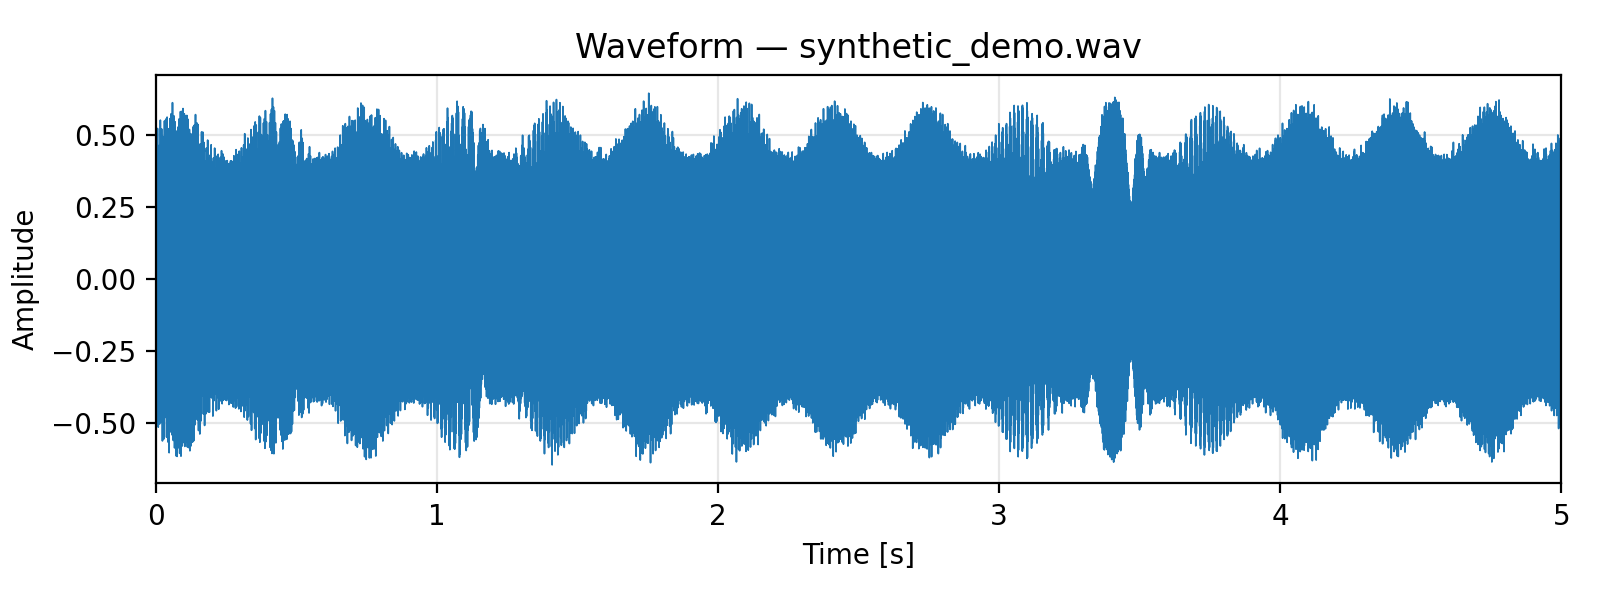
\includegraphics[width=\columnwidth]{../figures/synthetic_demo_waveform.png}
  \caption{Time-domain waveform of the 5-second synthetic test signal.}
  \label{fig:wave}
\end{figure}

\begin{figure}[!t]
  \centering
  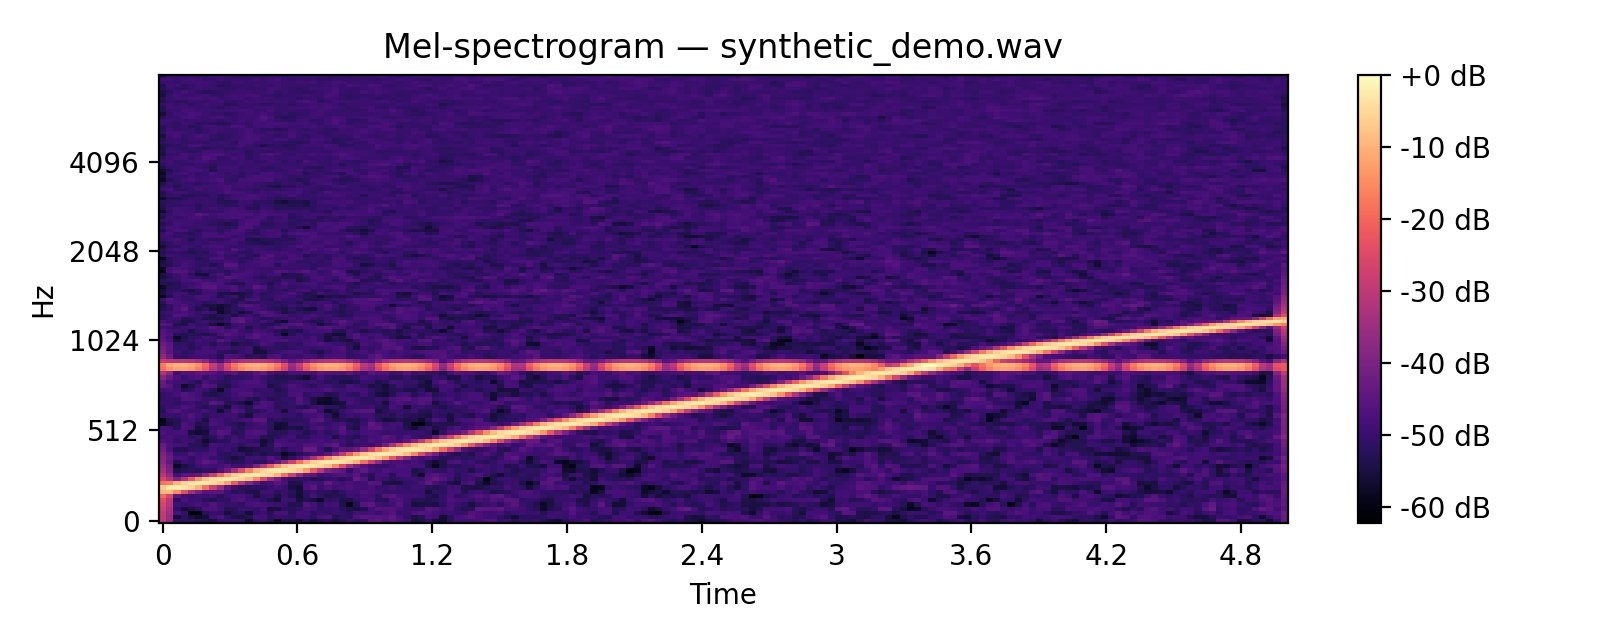
\includegraphics[width=\columnwidth]{../figures/synthetic_demo_mel.png}
  \caption{Log-amplitude mel-spectrogram (128 mel bins).
           The ascending diagonal is the chirp, the constant horizontal
           band is the AM tone.}
  \label{fig:mel}
\end{figure}

\begin{figure}[!t]
  \centering
  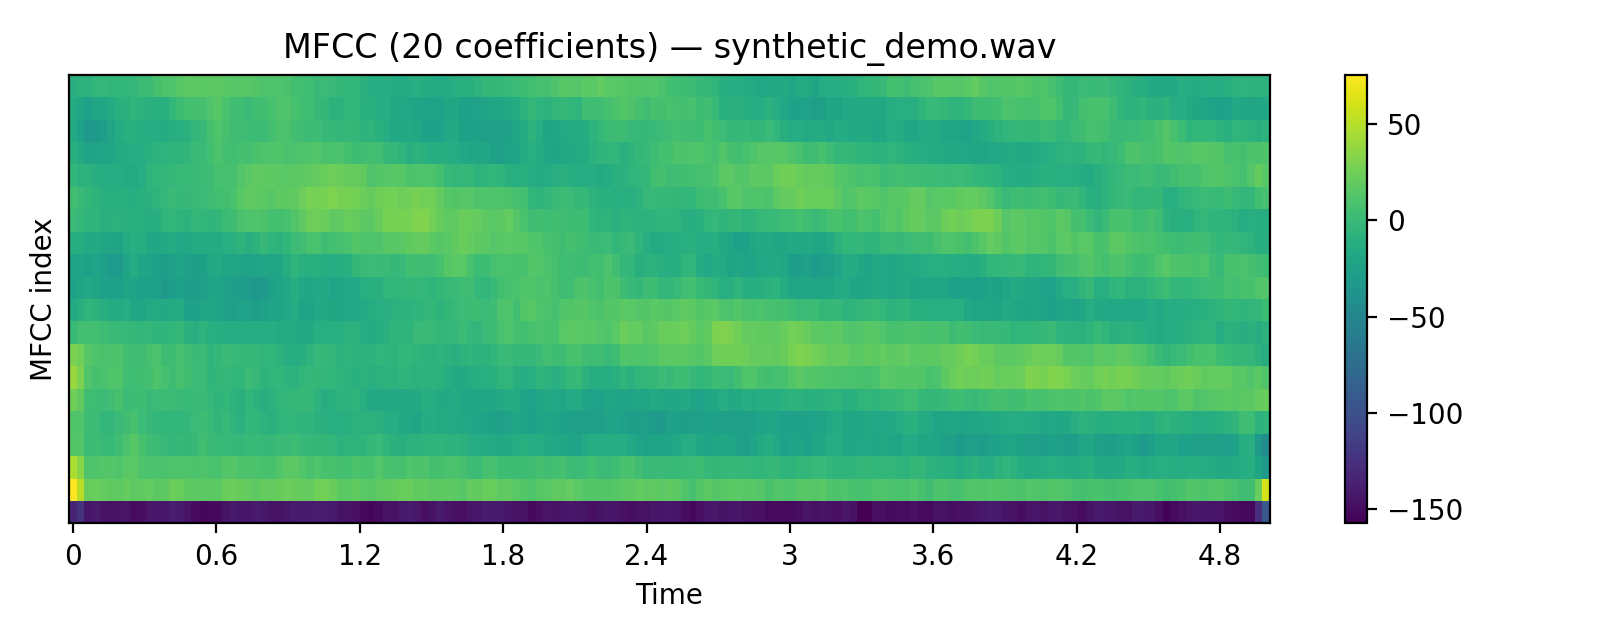
\includegraphics[width=\columnwidth]{../figures/synthetic_demo_mfcc.png}
  \caption{Twenty MFCC coefficients computed on the same signal.}
  \label{fig:mfcc}
\end{figure}

\begin{figure}[!t]
  \centering
  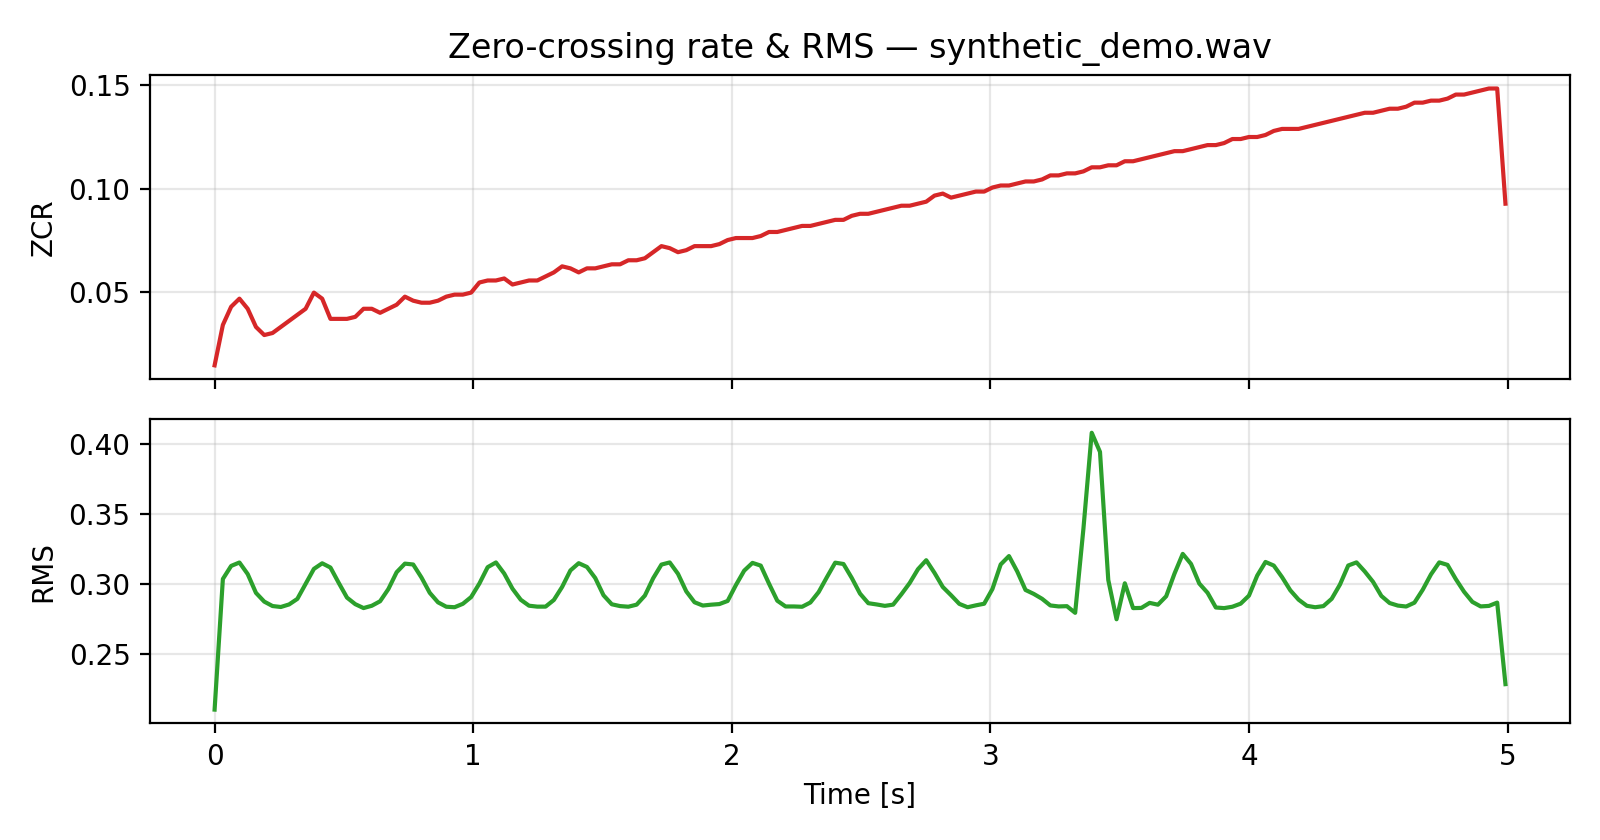
\includegraphics[width=\columnwidth]{../figures/synthetic_demo_zcr_rms.png}
  \caption{Zero-crossing rate (top) and short-time RMS energy
           (bottom) of the test signal.}
  \label{fig:zcr}
\end{figure}

\subsection{Compression Benchmark}
Table~\ref{tab:compression} and Fig.~\ref{fig:compression} compare the
three target codecs on the same synthetic clip
($156.3$\,kB original WAV, $16$\,kHz, $16$-bit, mono).  As expected,
FLAC is bit-exact (PSNR $=\infty$) at a $1.23\times$ ratio, MP3 at
64\,kbit/s achieves a $\approx 4\times$ ratio with $\sim 32$\,dB PSNR,
and OGG~Vorbis reaches $6.3\times$ at slightly higher PSNR than MP3
because Vorbis's psychoacoustic model is more aggressive on tonal
content.

\begin{table}[!t]
\caption{Round-trip compression metrics on a 5-second synthetic
         test clip (16~kHz, 16-bit, mono).}
\label{tab:compression}
\centering
\begin{tabular}{l r r r r}
\toprule
Codec & Bitrate & Size [kB] & Ratio & PSNR [dB] \\
\midrule
WAV   (source)        & ---  & 156.3 & 1.00$\times$ & $\infty$ \\
FLAC  (lossless)      & ---  & 127.4 & 1.23$\times$ & $\infty$ \\
MP3                   & 64\,k & 40.0  & 3.91$\times$ & 31.92 \\
OGG  (Vorbis)         & 64\,k & 24.8  & 6.30$\times$ & 34.04 \\
\bottomrule
\end{tabular}
\end{table}

\begin{figure}[!t]
  \centering
  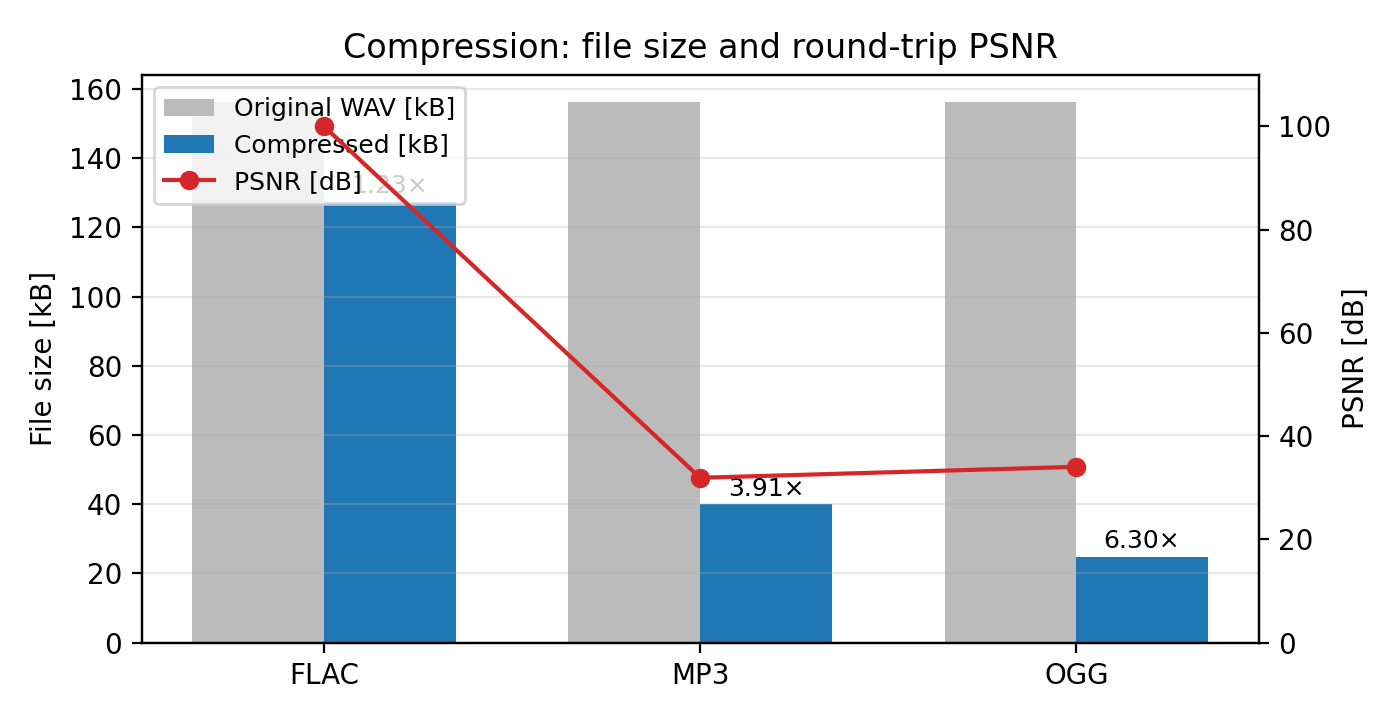
\includegraphics[width=\columnwidth]{../figures/compression_chart.png}
  \caption{File size (bars) and round-trip PSNR (red line) for the
           three target codecs.  FLAC's PSNR is clipped at the
           top of the right axis as it is mathematically infinite.}
  \label{fig:compression}
\end{figure}

\subsection{Reproducibility}
Every figure in this report can be regenerated with one command:
\begin{lstlisting}[language=bash]
$ python -m src.main demo
$ python src/make_compression_chart.py \
        outputs/compression.json \
        figures/compression_chart.png
\end{lstlisting}

% ============================================================================
\section{Conclusion}
% ============================================================================
The skeleton of the system is complete: Whisper transcription, four
spectro-temporal visualisations and three-codec compression all work on
synthetic audio with the metrics expected from the literature.  The
remaining work for the final demo is empirical -- running the pipeline
on real speech corpora, quantifying the compression-versus-WER trade-off
and (optionally) wrapping the CLI in a graphical front-end.

% ============================================================================
\begin{thebibliography}{9}
\bibitem{radford2022whisper}
A.~Radford \emph{et~al.}, ``Robust speech recognition via large-scale
weak supervision,'' \emph{OpenAI Tech.\ Rep.}, Sep.\ 2022.
[Online]. Available: \url{https://cdn.openai.com/papers/whisper.pdf}

\bibitem{hinton2012deep}
G.~Hinton \emph{et~al.}, ``Deep neural networks for acoustic modeling in
speech recognition,'' \emph{IEEE Signal Process.\ Mag.}, vol.~29,
no.~6, pp.~82--97, Nov.\ 2012.

\bibitem{davis1980comparison}
S.~B.~Davis and P.~Mermelstein, ``Comparison of parametric
representations for monosyllabic word recognition in continuously
spoken sentences,'' \emph{IEEE Trans.\ Acoust., Speech, Signal
Process.}, vol.~28, no.~4, pp.~357--366, Aug.\ 1980.

\bibitem{mcfee2015librosa}
B.~McFee \emph{et~al.}, ``librosa: Audio and music signal analysis in
Python,'' in \emph{Proc.\ SciPy}, 2015, pp.~18--25.

\bibitem{brandenburg1999mp3}
K.~Brandenburg, ``MP3 and AAC explained,'' in \emph{AES 17th Int.\ Conf.}
1999.

\bibitem{xiph2004vorbis}
Xiph.org Foundation, ``Vorbis I specification,'' Tech.\ Rep., 2004.
[Online]. Available: \url{https://xiph.org/vorbis/doc/Vorbis_I_spec.html}

\bibitem{coalson2008flac}
J.~Coalson, ``FLAC -- Free Lossless Audio Codec format,'' Xiph.org,
2008. [Online]. Available: \url{https://xiph.org/flac/format.html}

\bibitem{panayotov2015librispeech}
V.~Panayotov, G.~Chen, D.~Povey, and S.~Khudanpur, ``Librispeech: An
ASR corpus based on public domain audio books,'' in \emph{Proc.\ IEEE
ICASSP}, 2015, pp.~5206--5210.
\end{thebibliography}

\end{document}
